\documentclass[sn-mathphys-num]{sn-jnl}

\usepackage{graphicx}
\usepackage{multirow}
\usepackage{amsmath,amssymb,amsfonts}
\usepackage{amsthm}
\usepackage{mathrsfs}
\usepackage[title]{appendix}
\usepackage{xcolor}
\usepackage{textcomp}
\usepackage{manyfoot}
\usepackage{booktabs}
\usepackage{algorithm}
\usepackage{algorithmicx}
\usepackage{algpseudocode}
\usepackage{listings}
\usepackage{braket}

\raggedbottom

\begin{document}

\title[Article Title]{Quantum Oracles: How to Transform Classical Problems Into Quantum}


\author*[1]{\fnm{Alexandre} \sur{Silva}}\email{alexandresilvaunivem@gmail.com}

\author[2]{\fnm{Luis H.} \sur{Tobler Garcia}}\email{luishilario@univem.edu.br}

\author[3]{\fnm{Mauricio} \sur{Duarte}}\email{mauricio.duarte@fatec.sp.gov.br}

\affil*[1,2]{\orgdiv{Computer Science}, \orgname{UNIVEM}, \orgaddress{\street{Hygino Muzy Filho}, \city{Mar{\'i}lia}, \postcode{17525-901}, \state{S{\~a}o Paulo}, \country{Brazil}}}

\affil[3]{\orgdiv{Computer Science}, \orgname{FATEC}, \orgaddress{\street{Pres. Vargas}, \city{Gar\c{c}a}, \postcode{17400-000}, \state{S{\~a}o Paulo}, \country{Brazil}}}



\abstract{In this research, we provide a summary of all quantum Oracles that exists in the literature. Also, $5$ mini-projects were implemented trying to answer if it's possible to bring some classical problems to the quantum realm using these oracles as subroutines and data embedding providers. After finishing the tests, it was possible to see that, some of the implementations presented descent results. However, classical computing is still a fundamental part of quantum algorithms.}

\keywords{Quantum Computing, Algorithms, Quantum Algorithms, Oracles, Quantum Oracles, Problem Solving, Data Embedding}


\maketitle

\section{Introduction}\label{introduction}

Now days, it's not difficult to hear someone talking about quantum computers and how these machines will change the world. Nonetheless, the major fraction of these comments come from undue extrapolations and science fiction. In this paper, I'm going to show that quantum computing is not a magical trick to solve everything, but a tool for solving a distinct group of problems.
To do that, 5 mini-projects were implemented using Qiskit (\url{https://www.ibm.com/quantum/qiskit}), an open source quantum framework from IBM, exploiting quantum effects and using both pure quantum and hybrid approaches (classical + quantum algorithms) to reach the best results as possible, being then compared with their classical counterparts. Such mini-projects are the following: Quantum File explorer \ref{fileExplorer}, miles to kilometers conversion \ref{milesToKm}, Hanoi towers \ref{hanoiTowers}, Buckshot Roulette \ref{buckshotRoulette} and QROM/QRAM \ref{QRAM}. All the code were done in python and can be found at my GitHub repository (\url{https://github.com/Dpbm/scientific-initiation-1-quantum-oracles}).

\section{Oracles}\label{oracles}

Based on the idea of Oracle Turing Machines, the Oracles are mathematical modeling tools used to abstract outlying parts of an algorithm into a black-box, making its analysis much easier \cite{SOARE2009368} \cite{brodkorb_2019_the} \cite{davis_2006_turing} \cite{viswanathan_2013_reductions}. These machines could also be seen as a function, getting an input $x$ e returning $f(x)$ with time-complexity O(1). Due to this unreachable characteristics for real life, this model can't be classically implemented, being used only for formal description of decision problems \cite{kalyanasyndaram_2021_mod04lec23} \cite{amreen_oracle} \cite{e21080800}.
However, in quantum computing, it's possible to implement something similar to that, taking advantage of your inner structure and quantum effects to gain a relative speed-up to its classical counterparts as shown in the Deutsch-Jozsa's algorithm \cite{Fan_2007}. 

Furthermore, the Quantum Oracles have a fundamental role determining the complexity of a circuit. Some older methods are: depth, calculating the longest path in the circuit that some information must pass through; and gate counting, summing up how many gates were applied in the circuit. Although these methods are currently used, they are dependent of the QPU topology, differing from each backend used at transpilation time. As a solution, some parts of the circuit can be packed into Oracles and then its complexity calculated counting how many times they are called, also known as query complexity \cite{odonnell_2015_lecture} \cite{odonnell_2015_lecture_2} \cite{e21080800}.

\subsection{Types of Oracles}\label{oraclesTypes}

Knowing what Oracles are and where did they come from, we can classify them based on their structures and how the data is processed/encoded \cite{Kashefi_2002}.

\subsubsection{Phase Oracle}\label{phaseOracle}

The Phase Oracle, is the most well-known format. Some Algorithms, like Deutsch-Jozsa, Grover, Simon and Bernstein-Vazirani use it to take advantage over classical computing \cite{Fan_2007} \cite{bacon_2006_cse}.

As its main characteristic, the Phase Oracle adds a global phase to the circuit, using phase gates or quantum effects like Phase Kickback (the phase passes all the way through CNOT's target and is applied in the control qubit) to change values in superposition.

\pagebreak

\begin{figure}[ht]
	\centering
	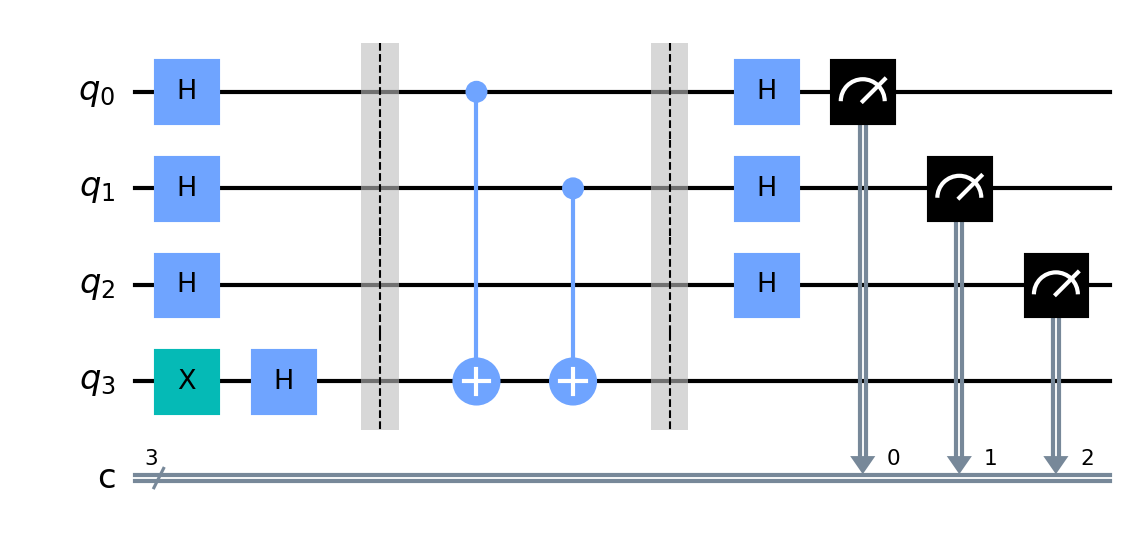
\includegraphics[width=0.9\textwidth]{assets/default_phase_oracle.png}
	\caption{Example of a Phase Oracle using Phase-Kickback. In this setup, an equal superposition is applied on qubits $q_{0\ldots2}$ and on the forth one (the auxiliary qubit), a $\pi$ phase is inserted in the form of a $\ket{-}$ state. This way, after applying $CNOT\ket{-}\ket{+}$, the state of these two qubits becomes ${\frac{1}{\sqrt{2}}}{(\ket{0}\ket{-} - \ket{1}\ket{-})}$, so after collapsing the superpositions at the end of the circuit, we reach the state ${\frac{1}{\sqrt{2}}}{(\ket{+}\ket{1} - \ket{-}\ket{1})}$, being $\ket{1}$ the new classical state for the control qubit. Doing that we can modify values that are within the superposition just interconnecting a phase with some state. This circuit is vastly known as the Deutsch-Jozsa's algorithm for a balanced Oracle. }\label{defaultPhaseOracleExample}
\end{figure}

It may seem useless, but it's possible to take advantage of this behavior and use it as a data encoding routine of which each time a $CNOT$ finds a $\ket{-}$ state acting on its target qubit, the base state for a superposition will be flipped on its control qubit.

Furthermore, there's another layout possible to implement a Phase Oracle. Once it only applies a phase in some bit-strings, the auxiliary qubit can be removed and the phase be provided by $CZ$ gates (or any other gate with phase application capabilities). Doing that, it's possible to create a Phase Oracle, keeping its unitary and reversible nature, in the format of a minimal Oracle.

\begin{figure}[ht]
	\centering
	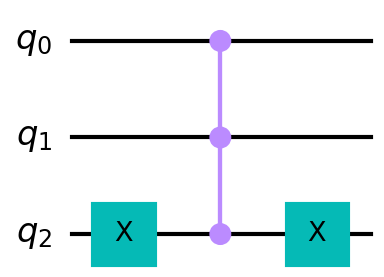
\includegraphics[width=0.4\textwidth]{assets/minimal_phase_oracle.png}
	\caption{Example of a Minimal Phase Oracle. This one uses a $MCP$ gate as a phase provider and two $X$ gates that were inserted to invert the qubits we want to have the value $0$, once the global phase is only added when every qubit is on $\ket{1}$ state. Doing that, this circuit applies a phase to the classical state $\ket{011}$ (little-endian), being a tiny example of classical to quantum data embedding.}\label{minimalPhaseOracleExample}
\end{figure}

\subsubsection{Boolean Oracle}\label{booleanOracle}

The Boolean Oracle has a similar structure with the previous one. However, in this case, it acts solely as a regular boolean function, mapping inputs to outputs.

\begin{figure}[ht]
	\centering
	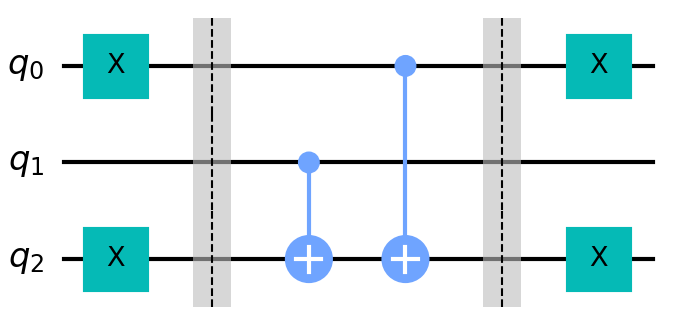
\includegraphics[width=0.7\textwidth]{assets/boolean_oracle.png}
	\caption{Boolean Oracle Example. The circuit shown is also know as the balanced oracle for the Deutsch-Jozsa's algorithm.}
	\label{booleanOracleExample}
\end{figure}


\subsubsection{Minimal Oracle}\label{minimalOracle}

As previously mentioned, the Minimal Oracle is a function which its essence is unitary and reversible, so no auxiliary qubits are required. Therefore, this format can be either Boolean or Phase Oracle, depending on its implementation.


\begin{figure}[ht]
	\centering
	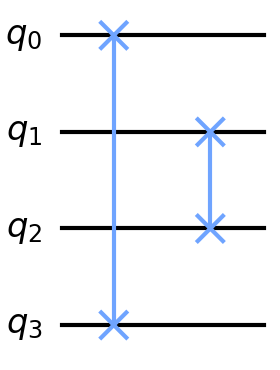
\includegraphics[width=0.3\textwidth]{assets/minimal_oracle.png}
	\caption{Boolean Minimal Oracle Example. Using two $SWAP$ gates, we invert the order of bit-strings in the unitary matrix, but no further modifications are done, so its unitary and reversible properties are kept, being a valid quantum operator.}
	\label{minimalOracleExample}
\end{figure}


\subsubsection{QFT(Quantum Fourier Transform)}\label{QFT}
The QFT is, in a nutshell, a quantum algorithm based on the Discrete Fourier Transformation, being used as quantum states period finding routine, projecting values from the computational basis onto the $X$ basis (also know as Fourier basis).

Even though it's an algorithm by itself, its application is done in the format of oracles for simplicity.

\begin{figure}[ht]
	\centering
	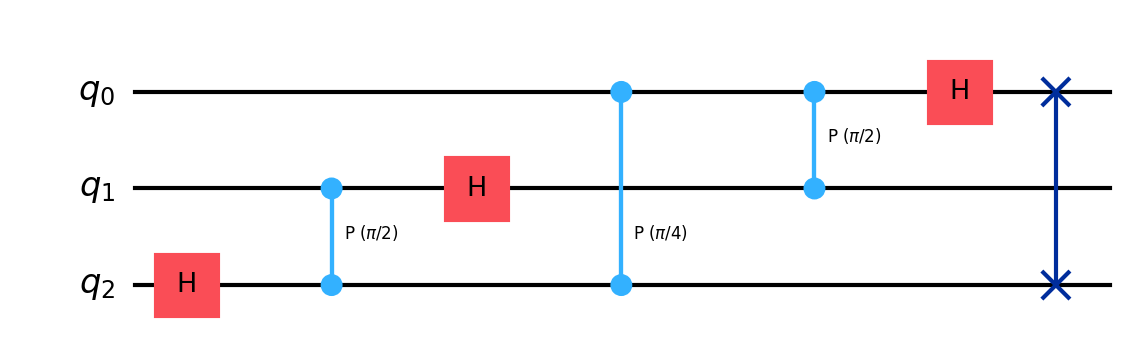
\includegraphics[width=0.9\textwidth]{assets/QFT.png}
	\caption{Quantum Fourier Transformation Oracle - Inner structure for $3$ qubits.}
	\label{QFTOracleExample}
\end{figure}

\subsubsection{Other kinds of Oracles}\label{otherOracles}

In addition to the oracles mentioned above, it's possible to come across with different mentions of Oracles, like Simons', Deutsch-Jozsa's, etc. However, these are just implementations of models already shown in this paper. Also, the most relevant for the incoming projects are both phase and boolean oracles. Due to that, there's no use of keeping discussing about many others sub-categories of oracles here.

\section{Development}\label{development}


\subsection{File Explorer}\label{fileExplorer}
Imagine a quantum computer, but instead of one of those we already have in real life, imagine a different kind, very similar to those we have at home, with a quantum operational system, quantum files, etc. This imaginary version could also be thought as a hybrid computer, taking advantage of both quantum and classical capabilities. 

Using this idea, the first project implements a file explorer for this ideal system.

The Standard solution for quantum search problems is the Grover's algorithm. This one realizes searches on unsorted "databases" (bit-string in this case) with $O(\sqrt{2^n})$, being $n$ the number of Qubits. Its tenets are based on amplitude amplification, using a Phase Oracle to mark the desired bit-strings and then using a Diffuser to amplify the probability of finding these values after measuring.

\pagebreak

\begin{figure}[ht]
	\centering
	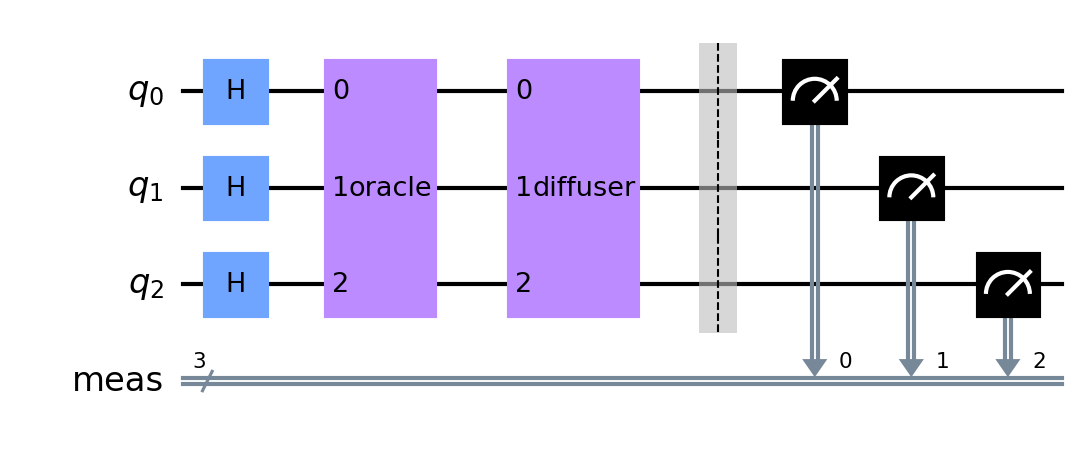
\includegraphics[width=0.9\textwidth]{assets/grover.png}
	\caption{Standard Grover's algorithm with $3$ qubits.}
	\label{GroverAlgorithmDefaultCircuit}
\end{figure}

To build the circuit, is needed a joint of $Oracle + Diffuser$ applied $k$ times, which $k \approx { {\frac{\pi}{4 \sqrt{\frac{a}{2^n}}}} - {\frac{1}{2}}  }$, being $a$ the number of values marked by the Oracle. Once we want to find just a single file, this relation is not required, being a single application all we need.

Although it's the best option for bit-string finding, in this project different rotations were tested trying to find a better superposition which increases the chances of finding the value we want.

\begin{figure}[ht]
	\centering
	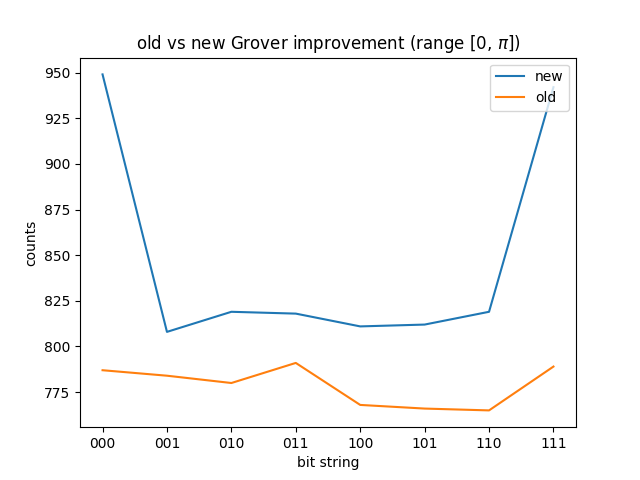
\includegraphics[width=0.8\textwidth]{assets/improvement_grover.png}
	\caption{Comparing the best superposition for each bit-string with Grover's default. At each iteration, the best rotation was found for each possible bit-string with $3$ qubits in the range $[0, \pi]$, then the outcomes were compared with the default rotation. In this case, as expected, the updated version overcomes the default one.}
	\label{GroverAlgorithmImprovement}
\end{figure}

\pagebreak

However, after comparing the best rotations with all bit-strings, the Grover's default superposition is the best in general.

\begin{figure}[ht]
	\centering
	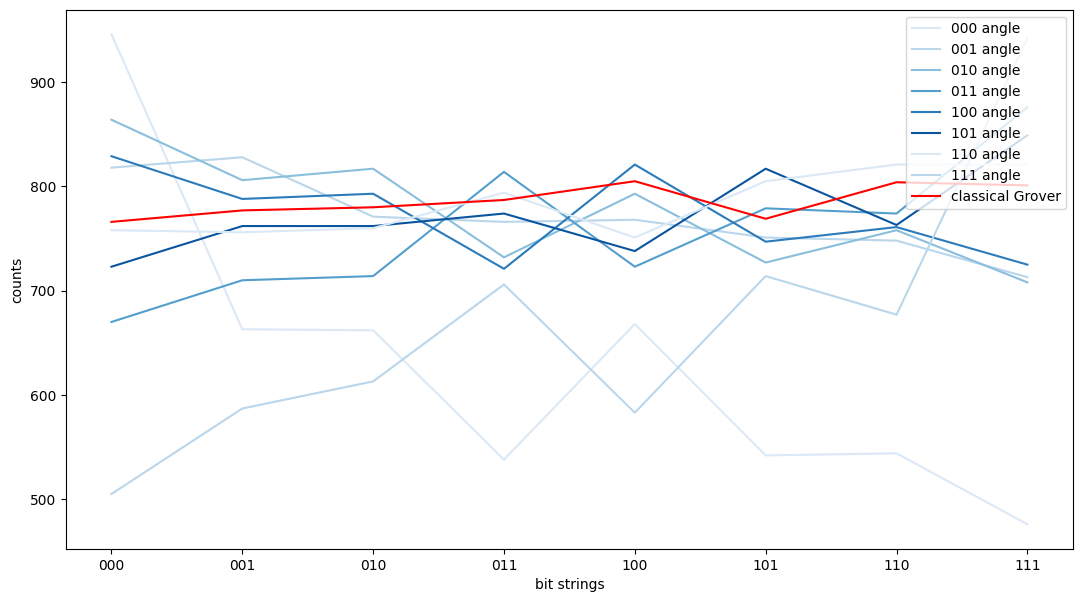
\includegraphics[width=0.9\textwidth]{assets/especific_rotations_compare.png}
	\caption{Testing every bit-string optimal rotation over all the search space. With this test, is possible to see that the standard half superposition is the best on average, being good for every bit-string in a more general case, but not optimal every single one.}
	\label{GroverAlgorithmRotationsComparation}
\end{figure}

For the purpose of this project and experimentation, a hybrid approach was used. This way, during the circuit setup, the searched value pass
through a hash-table with optimal angles that will be used as a rotation in the beginning of the circuit. Doing that, the chances of finding the file we want are increased optimally.

With this setup, we have the search algorithm ready to work, but it's still required a way to get from the quantum hard-drive the files we want. 

Solving this issue is quite simple, it's possible to exploit the behavior of overlapping two phase oracles, remaining only the difference between these two (as sets difference on math as shown at \cite{sanchezrivero2023initial}).

To implement this algorithm step-by-step, we need to:

\begin{enumerate}
	\item{Pass the desired bit-string through the hash-table}
	\item{Use the optimal angle to initialize the equal superposition on the qubits}
	\item{Apply the Phase-Oracle that encodes all the files (bit-strings) available on disk}
	\item{Apply the Inverse Phase-Oracle that encodes all the files except those we want to find}
	\item{Apply the Diffuser}
	\item{Measure $n$ times}
\end{enumerate}

\pagebreak


The resulting algorithm seems like this for $3$ qubits.

\begin{figure}[ht]
	\centering
	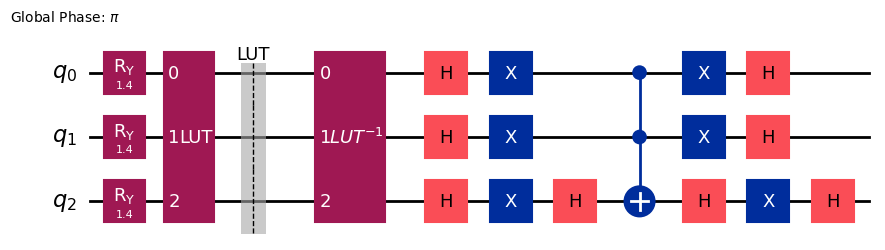
\includegraphics[width=0.9\textwidth]{assets/file_explorer.png}
	\caption{Implementation of the described quantum file explorer for $3$ qubits.}
	\label{FileExplorerAlgorithm}
\end{figure}

As a conclusion for the very first project, it's so far the best known setup to search between "quantum files" for this hypothetical scenario. However, it can't be seem as a best known solution ever, once even classical approaches using trees can beat the current $O(\sqrt{N})$ of Grover's algorithm.
Also, it's very expensive to keep track of all optimal rotations in a hash-table due to the exponential growth of bit-string combinations at each qubit addition. For this case, using the pure Grover's algorithm can be a best solution, but it's still worse than its classical counterparts.

\subsection{Miles To Kilometers Conversion}\label{milesToKm}

The second problem tackled here was the conversion from miles to kilometers. This idea came out after reading the description of a quantum Fibonacci algorithm at \cite{gilliam2020canonical}. Once the miles to kilometers relations can be approximated using the Fibonacci sequence \cite{usman_2019_kilometres}, theoretically it's possible to use the given circuit to do the same in a quantum manner.

For this algorithm, it's required a circuit with $n$ qubits, being $n$ also the $n$-th number of the sequence starting from $2$. The implementation starts with an equal half-superposition throughout the qubits, and then controlled $RY$ rotations by $-\frac{\pi}{2}$ are applied linearly until the last qubit. This algorithm isolates bit-strings that contains consecutive ones letting only the other ones to pass, so after $m$ measurements, it's presented a distribution of bit-strings and, with some post-processing, we can count those bit-strings that shown-up in the distribution, giving the value of $F(n)$.

\pagebreak

\begin{figure}[ht]
	\centering
	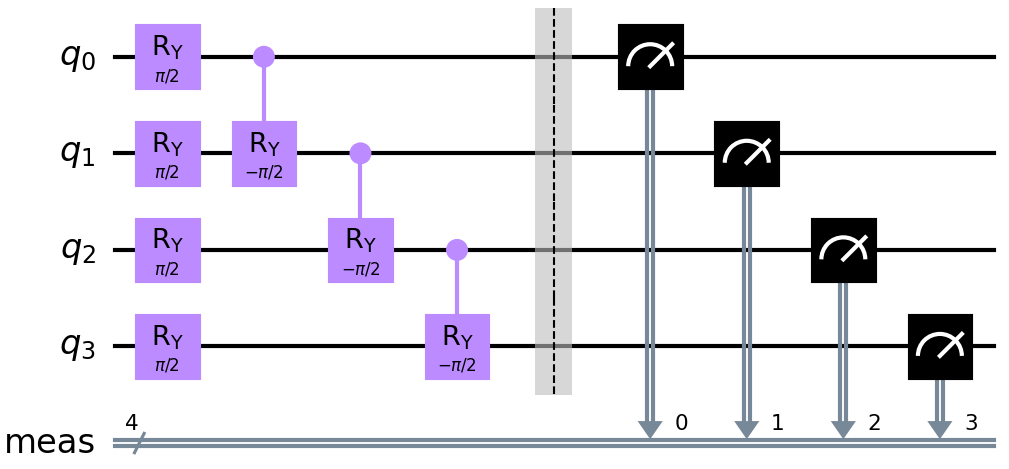
\includegraphics[width=0.8\textwidth]{assets/fibonacci.png}
	\caption{Quantum Fibonacci for $4$ qubits. It's expected to obtain $F(4)=8.$}
	\label{fibonacciExample}
\end{figure}
  
\begin{figure}[ht]
  	\centering
  	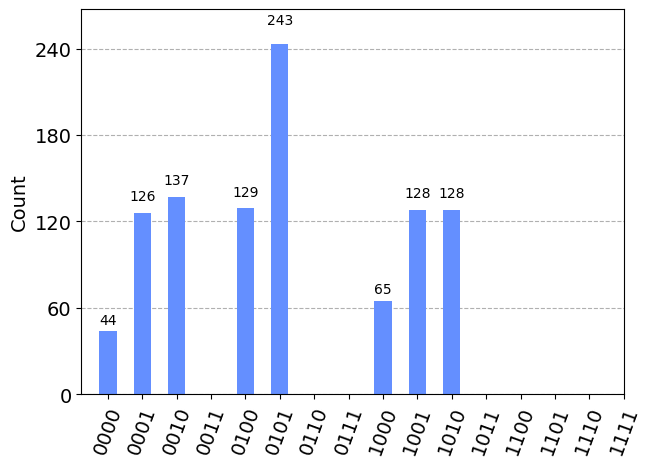
\includegraphics[width=0.8\textwidth]{assets/fibonacci_result.png}
  	\caption{Measurement results after $1000$ shots on a Qiskit AER simulator. In this example, it's possible to see that multiple bit-strings haven't shown up and, as expected, are those with consecutive ones. So, the algorithm worked, now after counting the how many bit-string appeared at the end we have the result of $F(n)$. In this case, $8$ bit-strings were in the distribution with non-zero count, so $n=4$ and $F(4) = 8$ as we foreseen. During this setup, it must be bared in mind that the sequence for this quantum version starts at $2$ so $F(1)=2, F(2)=3, F(3)=5, F(4)=8, F(5)=13, F(6)=21, \ldots$.}
  	\label{fibonacciResultExample}
\end{figure}


Looking closely at those results and pairing it with the relation between kilometers and miles, can be seen a clear relation between Fibonacci results and the approximated kilometers values.

\pagebreak

\begin{table}[ht]
	\caption{Classical Conversion relation}\label{conversionRelation}%
	\begin{tabular}{@{}lll@{}}
		\toprule
		miles & $\approx$ Km & Real(Km)\\
		\midrule
		1 & 2 & 1.60934\\
		2 & 3 & 3.21869\\
		3 & 5 & 4.82803\\
		5 & 8 & 8.04672\\
	\end{tabular}
\end{table}

So, to convert the desired miles value, the equation $F_{km} = F_{miles}(n+1)$ is the perfect match for known values in the sequence, requiring the next $n$ for the conversion. Although some values can be already converted, it's useless for those outside Fibonacci's series. For these cases, a solution is split the number into Fibonacci factors and then sum them up at end so, for instance, transforming $10$ miles to kilometers is the same as summing the resulting values of the above equation for $F(5)=8$ and $F(2)=2$ resulting in $F(5 + 1) + F(2 + 1) = F(6) + F(3) = 13 + 3 = 16Km$.

Using that idea, a quantum circuit could be easily done taking advantage of hybrid computation and mid-circuit measurements to retrieve the distributions at execution time. This way, the final algorithm breaks down the input miles value into smaller factors, applies the oracle that embeds the Fibonacci for that specific $n$, measure $m$ times and then reset for the next application. Once a same factor can be used multiple times for a same input value, we can squeeze this algorithm removing duplicated oracles and just multiplying the results at end by how many times that factor should have been calculated $i$. This final setup can be expressed algorithmically as:

\pagebreak

\begin{algorithm}
	\caption{Quantum Miles to Kilometers Conversion Algorithm}\label{quantumConversion}
	\begin{algorithmic}[1]
		\State parts = $BreakInputIntoFibonacciParts(input)$
		\For{part in parts}
			\State Apply the Oracle embedding $F(part)$
			\State Measure the Oracle Qubits
			\State Reset these Qubits
		\EndFor
		\State Parse the results from the outcomes distributions
		\State Calculate $\sum_{i=0}^{N} {o_{i}p_{i}}$, where $N$ is the total of split parts and $o$ the outcome
	\end{algorithmic}
\end{algorithm}


\begin{figure}[ht]
 	\centering
 	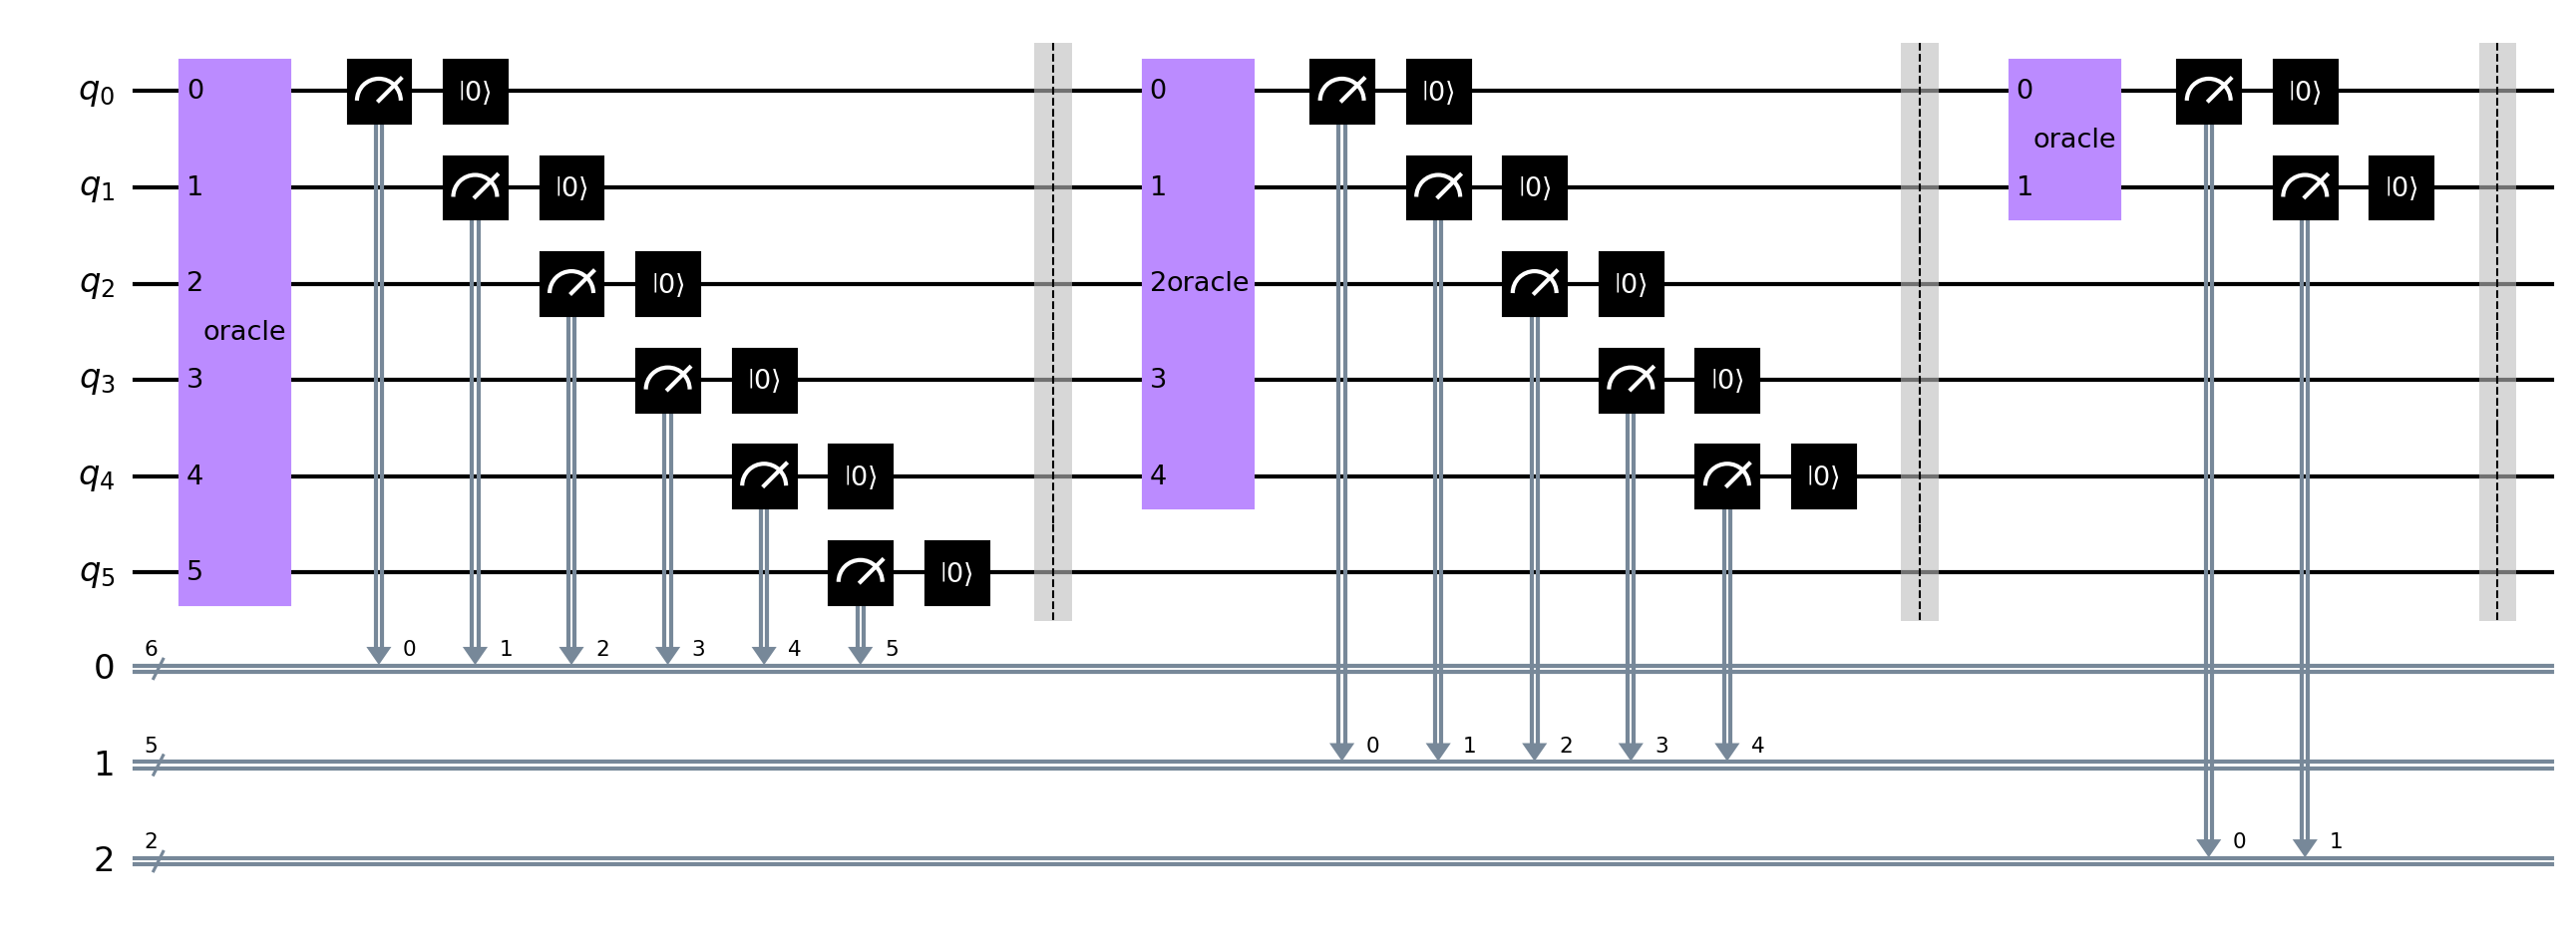
\includegraphics[width=1\textwidth]{assets/conversion_circuit.png}
 	\caption{The final conversion quantum algorithm. The circuit, consists of a quantum register with the maximum number of qubits required and one classical register for each oracle measurement.}
 	\label{quantumConversionAlgorithm}
\end{figure}

After testing this method for a bunch of different input values, the conclusion is that it truly works. However, as the input grows, the divergence between the correct values grows as well.

\pagebreak

\begin{figure}[ht]
	\centering
	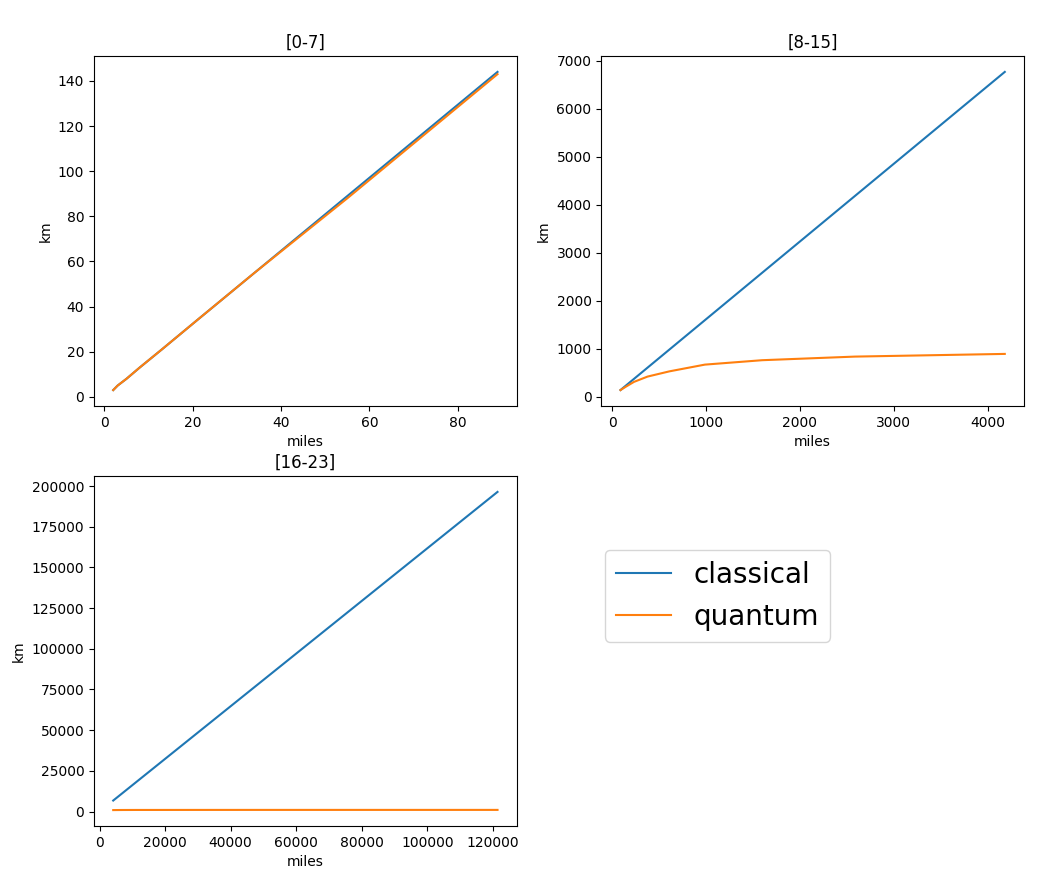
\includegraphics[width=1\textwidth]{assets/conversion_tests.png}
	\caption{Comparing the correct values with the quantum version outputs. For this test, as the classical results grew linearly as expected, the quantum ones started to diverge badly giving nonsense returns.}
	\label{qauntumConversionTests}
\end{figure}

Then, after implementing this project, the conclusion is that it's possible to use Fibonacci approximation in quantum circuits, however it's not worth it, once there's too much classical overhead in it and, at some point, the resulting values may diverge completely from what it was expected to be. Saying that, this algorithm can't surpass its classical approach, at least when following the setup above.

\subsection{Hanoi Towers}\label{hanoiTowers}

Hanoi Towers is a classical computing problem, vastly used in computer science to teach about recursion and problem solving \cite{ldiaandr_2021_tower} \cite{diptokarmakar47_2019_how} \cite{a2020_towers}. The goal for this mini-project is to mimic the classical behavior and solve the towers.

To reach this goal, a phase oracle is used to embed the disks positions on the rods, then $SWAP$ gates are applied to move them from a rod to another. The disks, in this configuration, are the bit-strings, which are divided evenly by $3$ distinct quantum registers with the same number of qubits. These registers are meant to be the representation of binary rods, this way, a rod with $3$ qubits can represent, at most, $2^3=8$ disks. Also, the disposition between them are the same as the classical, being the first one the source rod, the second an auxiliary and the third one the target $\ket{t_{n-1} t_{n-2} ... t_0}\ket{a_{n-1} a_{n-2} ... a_0}\ket{s_{n-1} s_{n-2} ... s_0}$.
For the sequence o $SWAP$ gates, first the movements must be pre-calculated classically \cite{geeksforgeeks_2014_program} and next be applied for each qubit in the circuit.

\begin{figure}[ht]
	\centering
	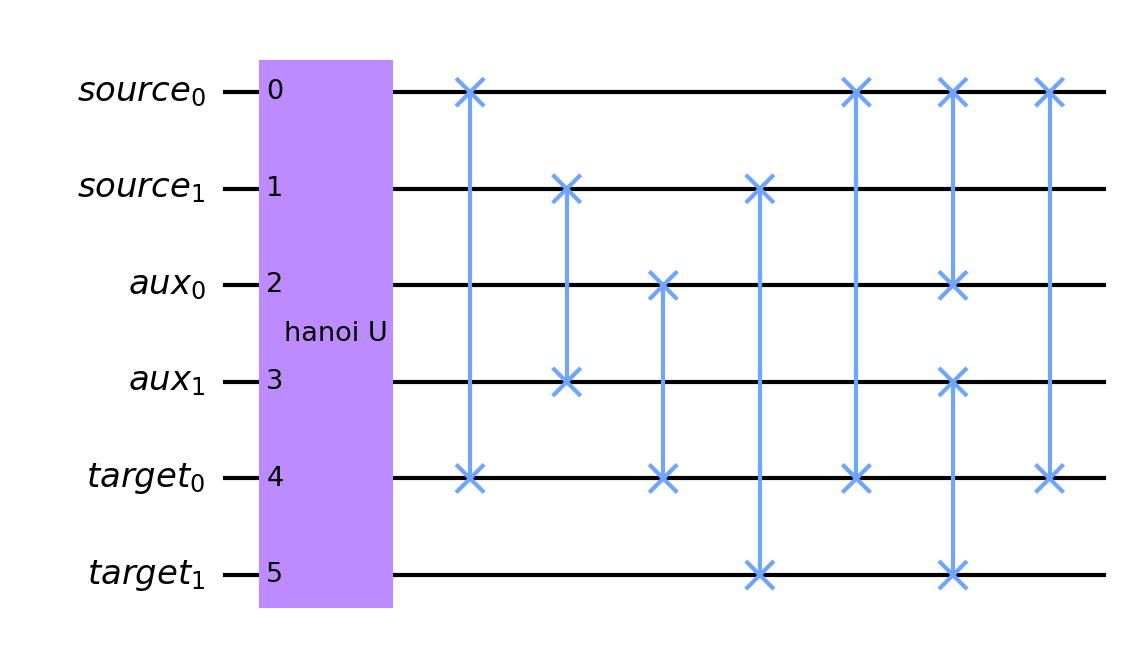
\includegraphics[width=0.9\textwidth]{assets/hanoi_circuit.png}
	\caption{Quantum Hanoi Towers for $3$ disks. Inside its Oracle, the values $000001$, $000001$ and $000011$ are encoded representing each disk respectively from $1$ to $3$ on the source rod.}
	\label{hanoiCircuit}
\end{figure}

The circuit itself can't provide any results after measurements, for that is required a supplementary algorithm to get the amplitudes, like Grover's Diffuser.

\pagebreak

\begin{figure}[ht]
	\centering
	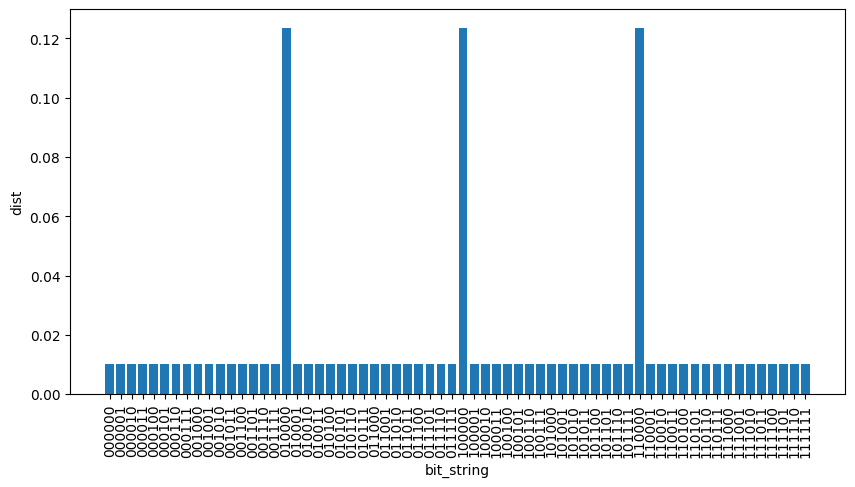
\includegraphics[width=1\textwidth]{assets/hanoi_results.png}
	\caption{Quantum Hanoi Towers with $3$ disks after amplitude amplification with Grover's algorithm. In these results, the $3$ most likely bit-strings are $010000$, $100000$ and $110000$ which show us that the disks went correctly from the source register (the right-most qubits) to the target register (the left-most qubits).}
	\label{hanoiResults}
\end{figure}

Even thought the whole quantum algorithm is based, most part, on classical routines, it doesn't reduce its usability compared to its equivalents in classical computing. It's evident when we keep in mind that classically, it's required to first get the next movement before you play. Saying so, both cases share the same core, being equivalent.

\subsection{Buckshot Roulette}\label{buckshotRoulette}

\textit{Buckshot Roulette} is a computer game made by \textit{Mike Klubnika}(\url{https://mikeklubnika.itch.io/}), based on the idea of modifying the infamous Russian Roulette.
During the game, you are challenged to play against a demon (dealer). If you win, you'll receive a prize, otherwise the game will restart and you can try again.

The game itself has many rounds with a vast range of power-ups but, for this very project, we analyzed only the first match, trying to find the best strategy to maximize the player's winnings. The reason for this choice is due to its simplicity, being away from power-ups that could complicate the analysis while maintaining the dynamics that's hold during the entire game.

During the first match, $2$ fake bullets and $1$ real are put into a shotgun. Then, the player starts his play, choosing either shooting himself or his opponent. If the player shoots himself and it's a real bullet, he loses one life point, otherwise he gets another chance to choose. However, if he chooses to shot his opponent, if it's real he takes away one life point from him, otherwise his opponent receives the gun. To understand it better, the dynamics can be modeled as a tree following the game theory methods \cite{sep-game-theory}.

\begin{figure}[ht]
	\centering
	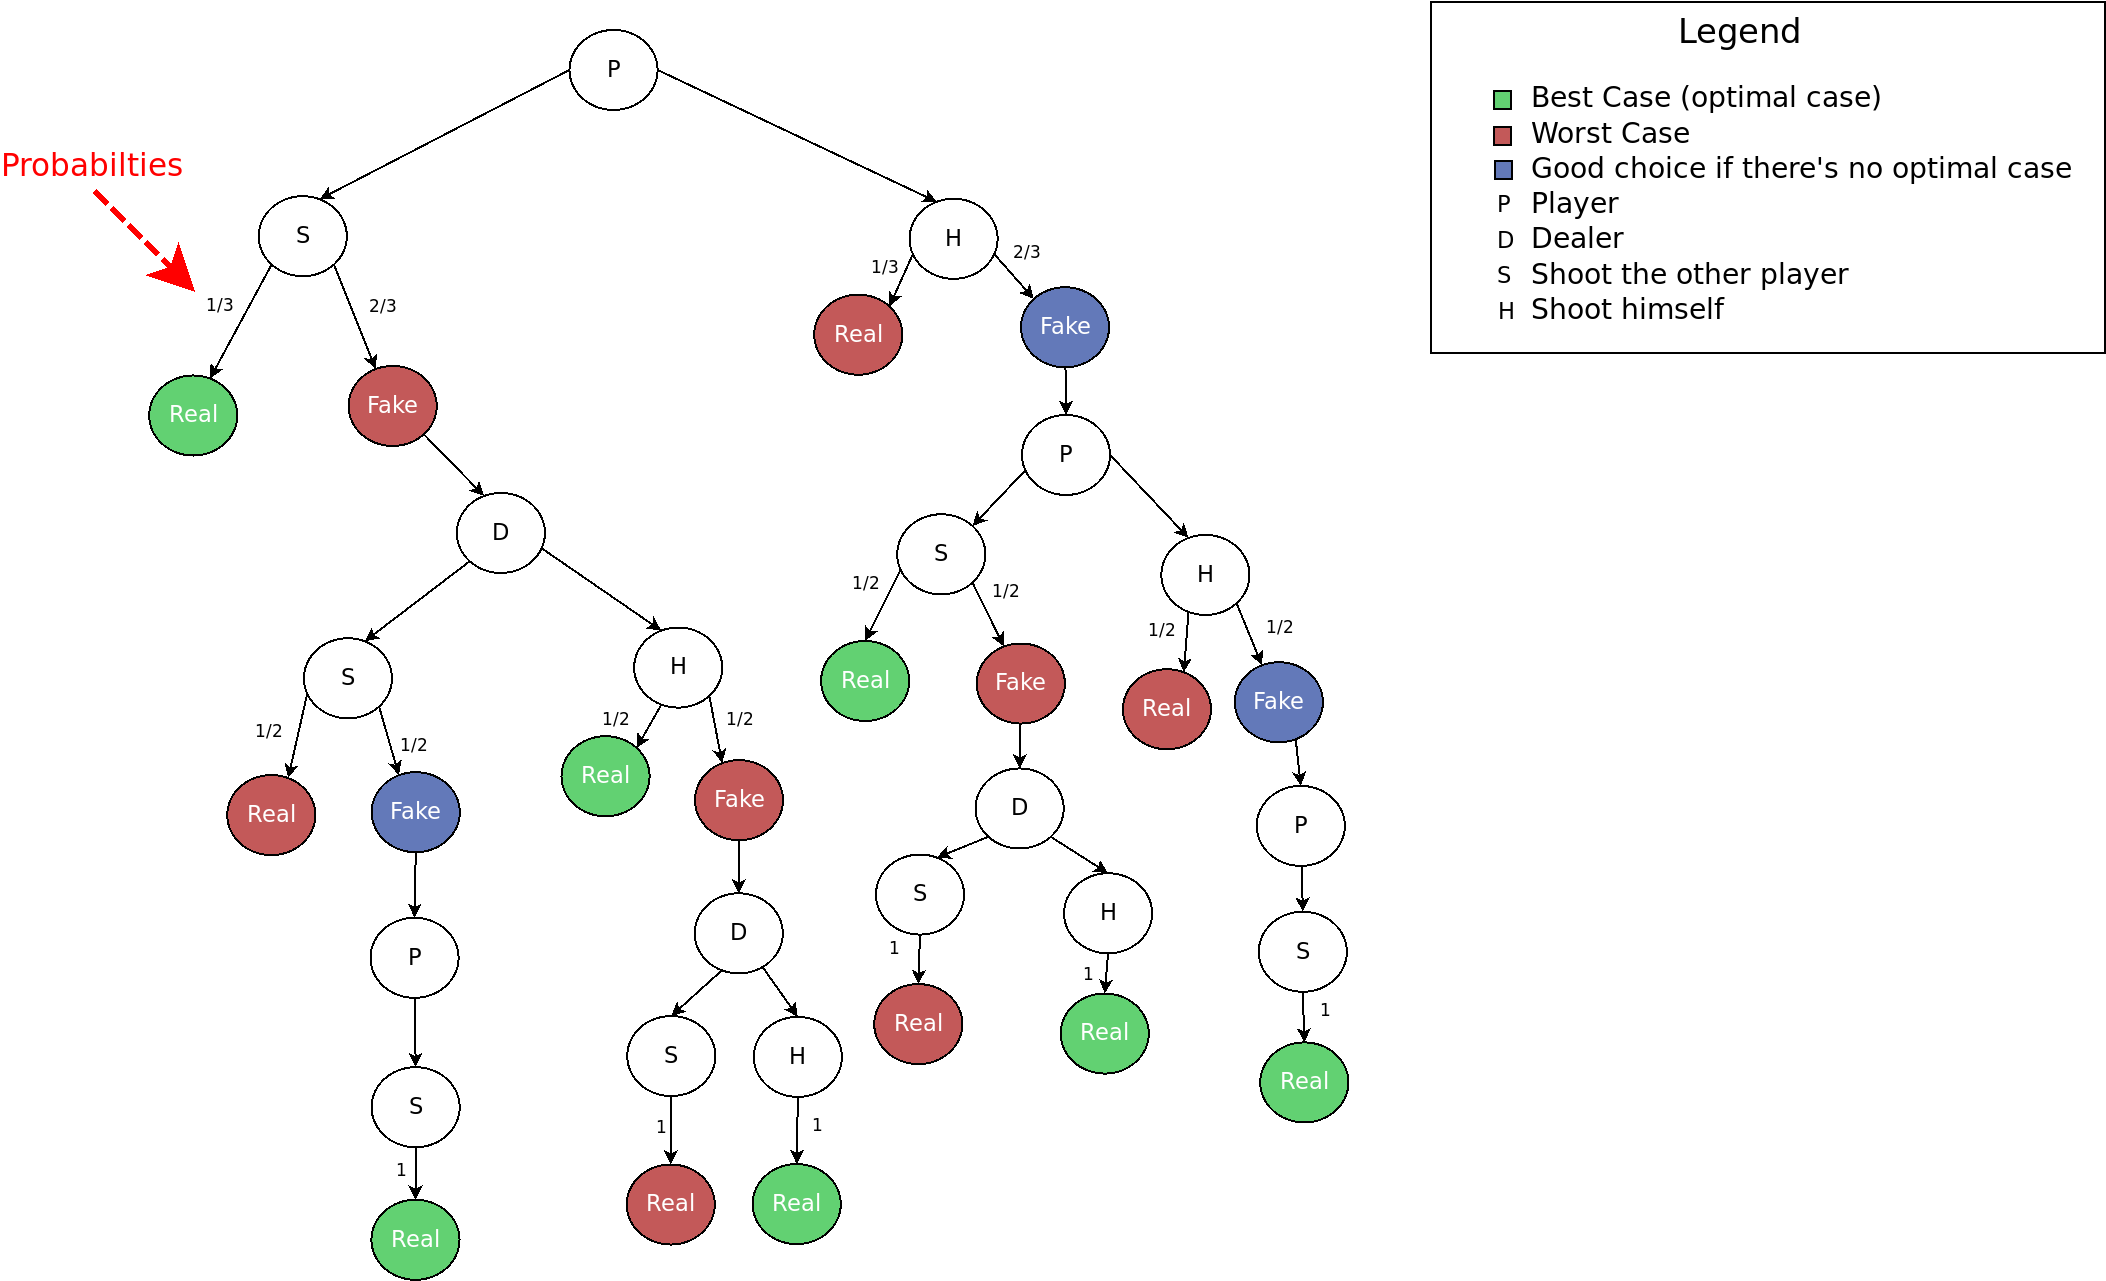
\includegraphics[width=1\textwidth]{assets/buckshot_roulette_diagram.png}
	\caption{Buckshot Roulette Tree Diagram expressing the probabilities for players future paths. For this diagram, it's expected that the player is a rational agent, which always plays aiming to win, and the dealer is a random agent, choosing randomly his decisions. Due to that, it's possible to see that the leafs which were reached by the player, have only one possible value "Shoot", once both of them are alive and clearly on the gun has a real bullet waiting to shot; but those reached by the dealer have two, either "Shoot himself" or "His opponent" due to his lack of memory and reasoning.}
	\label{buckshotRouletteDiagram}
\end{figure}

Following the paths, we can create an algorithm to simulate this game multiple times and then try to find the best solution.

After testing multiple possible paths, the best one was given by the path which the player starts shooting the dealer.

Analyzing this strategy, the conclusion is that, this is the best strategy because the player has less chances to die, once he doesn't have the chance of killing himself right at the beginning.

\begin{table}[ht]
	\caption{Player starts shooting himself path}\label{playerStartsShootsHimselfPath}%
	\begin{tabular}{@{}llll@{}}
		\toprule
		Bullet & Action & Action Result & Result \\
		\midrule
			1 & player shoots himself  & real & dealer wins\\
			1 & player shoots himself  & fake & -\\
			2 & dealer shoots player  & real & dealer wins\\
			2 & dealer shoots player  & fake & -\\
			2 & dealer shoots himself  & real & player wins\\
			2 & dealer shoots himself  & fake & -\\
			3 & player shoots dealer  & real & player wins\\
			3 & dealer shoots player & real & dealer wins\\
			3 & dealer shoots himself & real & player wins\\
	\end{tabular}
\end{table}

\begin{table}[ht]
	\caption{Best strategy path}\label{bestStrategyPath}%
	\begin{tabular}{@{}llll@{}}
		\toprule
		Bullet & Action & Action Result & Result \\
		\midrule
			1 & player shoots dealer  & real & player wins\\
			1 & player shoots dealer  & fake & -\\
			2 & dealer shoots player  & real & dealer wins\\
			2 & dealer shoots player  & fake & -\\
			2 & dealer shoots himself  & real & player wins\\
			2 & dealer shoots himself  & fake & -\\
			3 & player shoots dealer  & real & player wins\\
			3 & dealer shoots player & real & dealer wins\\
			3 & dealer shoots himself & real & player wins\\
	\end{tabular}
\end{table}

As in \ref{playerStartsShootsHimselfPath} the player starts shooting himself, on total he has only $3$ possibilities of winning. On the other hand, as shown in \ref{bestStrategyPath}, the player has in total $4$ chances of winning, being the best strategy for him.

After finding the best classical result, the next step is translate that to a quantum circuit. For this new version, each player is represented as an oracle, embedding their strategies inside as a Bloch Sphere rotation. The gun, in this case, is a half-superposition gate, letting it fires $50\%$ of the time no matter how many bullets are there. Then, these are placed on a circuit that mimics the game actions and the final bit-strings are evaluated. By the end of this simulation, those angles embedded inside the human player's oracle are changed aiming to maximize his gains.

\pagebreak


\begin{figure}[ht]
	\centering
	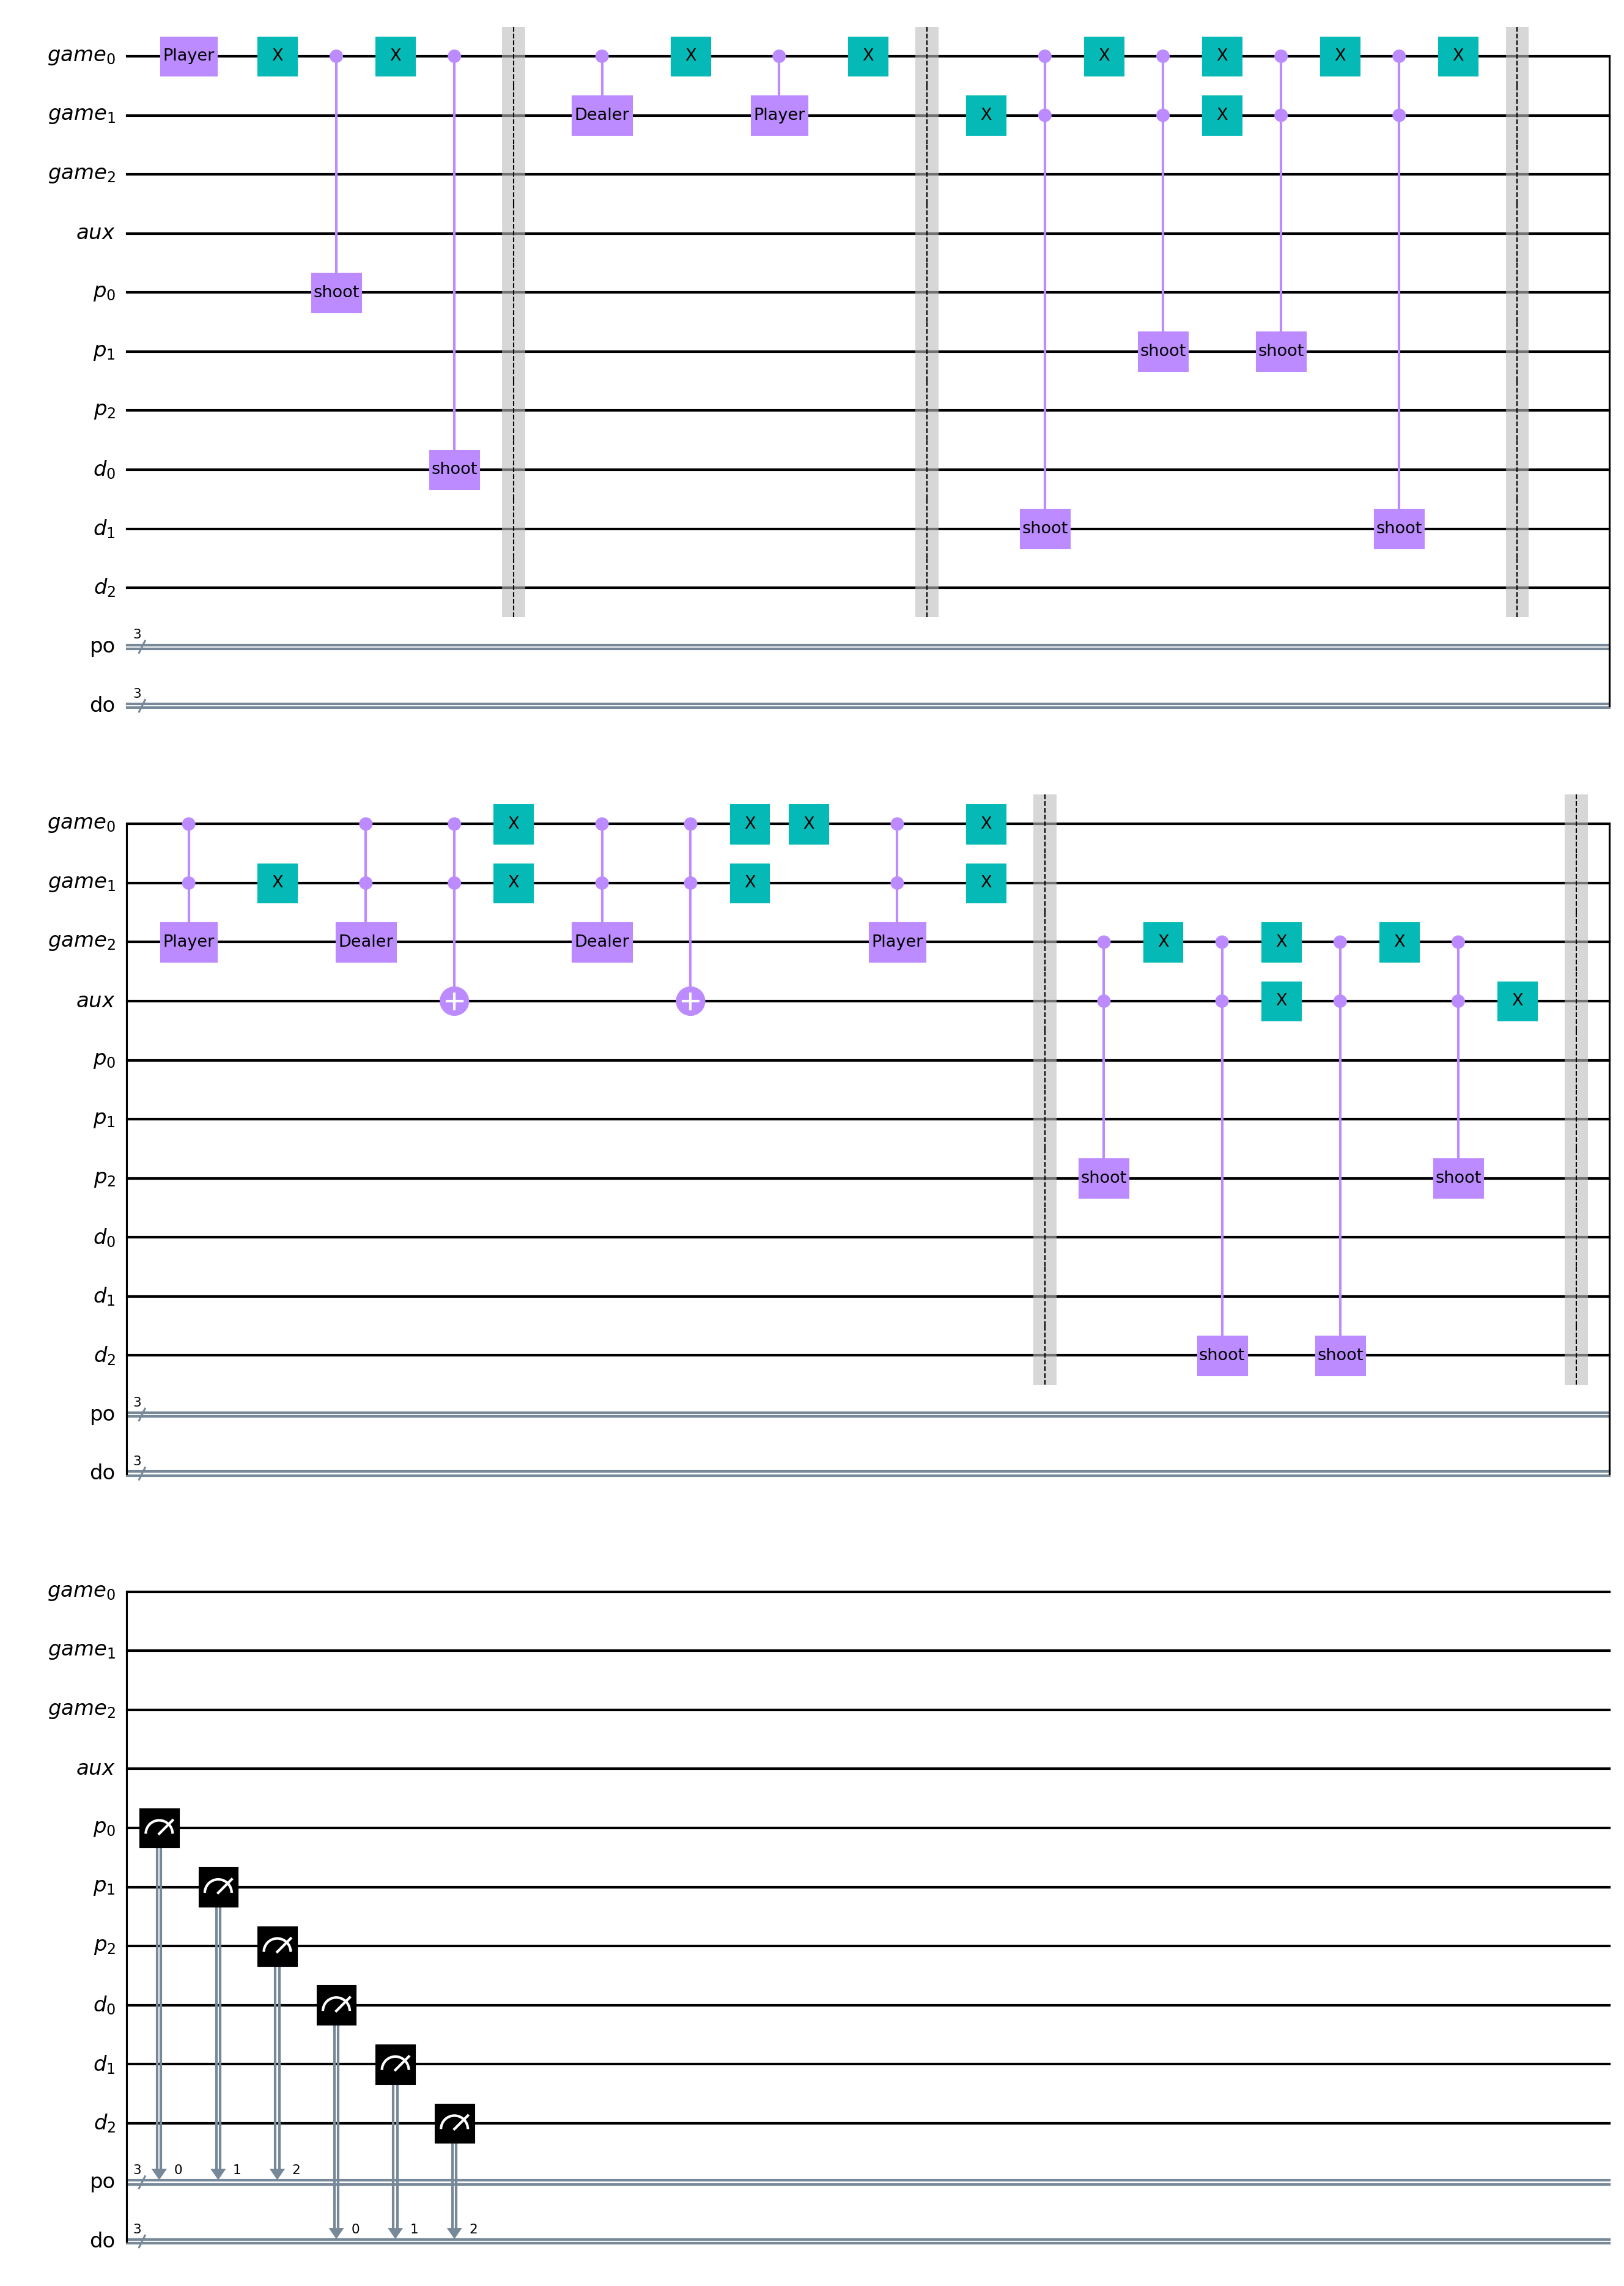
\includegraphics[width=0.8\textwidth]{assets/quantum_buckshot_roulette.png}
	\caption{Quantum Buckshot roulette circuit.}
	\label{buckshotRouletteCircuit}
\end{figure}

The rotation angles used here are $\theta$ and $\phi$, so phases can be also explored.
Finishing the evaluation process, those angles that returned the best results are: $\theta\approx 3.0853981633974477, \phi\approx3.7853981633974474$ radians. Plotting them on a Bloch Sphere, it confirms our classical projection, the player has always the tendency of shooting his opponent (bit $1$) instead of himself (bit $0$), being the optimal strategy as found classically.

\pagebreak

\begin{figure}[ht]
	\centering
	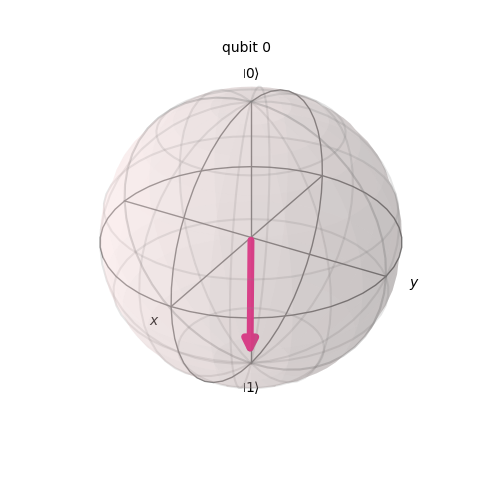
\includegraphics[width=0.5\textwidth]{assets/quantum_buckshot_roulette_strategy.png}
	\caption{Quantum Buckshot Roulette player's optimal results. As expected, the player tends to shoot his opponent whenever he can (state $\ket{1}$).}
	\label{buckshotRouletteQuantumStrategy}
\end{figure}

\begin{figure}[ht]
	\centering
	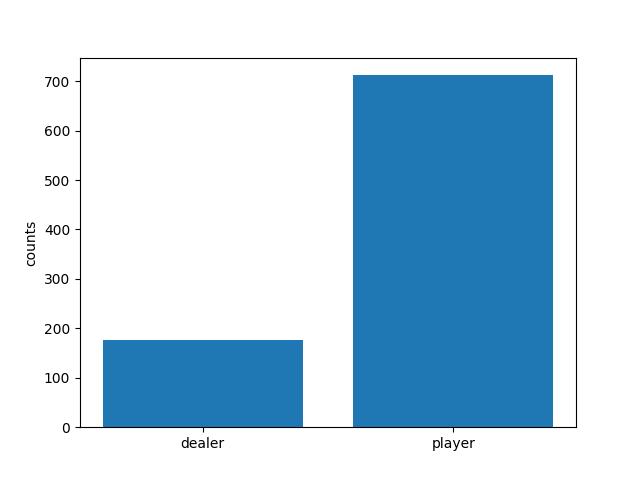
\includegraphics[width=0.6\textwidth]{assets/quantum_buckshot_roulette_results.png}
	\caption{Results of the simulation for quantum buckshot Roulette. Using the optimal strategy, the player can excel the dealer's results only by choosing to shoot every time that's possible.}
	\label{buckshotRouletteQuantumResults}
\end{figure}

For this problem, once our goal in it is to find the best strategy, there's no way to say which one is better wether quantum or classical version. However, in a more theoretical game theory view, the quantum version can get advantage of some effects, like entanglement, superposition and interference, which can leads to better results \cite{frackiewicz2011application} \cite{Eisert_1999} \cite{khan_2021_quantum} \cite{legn_2022_dilemma} \cite{vijayakrishnan_2019_role}.

In general, both simulations reached the same result and it was shown that it's possible to model and simulate a game with quantum circuits using Oracles as player's strategies representations.

\subsection{QRAM and QROM} \label{QRAM}

Finally, the last project done was a QRAM/QROM based on Quantum Oracles. Here, a QROM with static data was tested as well as a QRAM able to read/write data from inside.
Differing from most part of researches on these devices \cite{Giovannetti_2008}, in this paper the goal is to store all kinds of quantum states, not only bit-strings. The reason for this choice is the real application for this sort of appliance. If someday a QRAM becomes real, its maximum power would be only reached when its capabilities enable the storage of superposition states \cite{siegelwax_2022_quantum}.

To start the implementations, a QROM was designed with $n$ Qubits being used for the address bus and $m$ for the data bus however, these numbers don't share any correlations, so it's possible to have a configuration like $n = 3; m = 10$. This happens due the address mapping circuit, which when some bit-string is inserted on its bus, controlled gates are used to handle the input and map it to the desired state, so the whole application can be done with more than one gate and more than one target qubit.

\begin{figure}[ht]
	\centering
	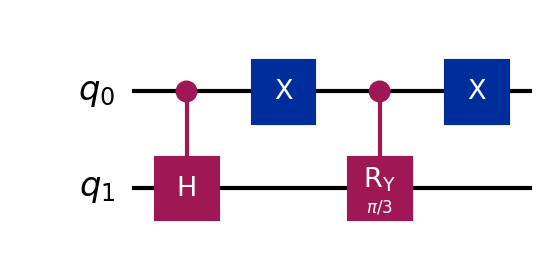
\includegraphics[width=0.9\textwidth]{assets/qrom.png}
	\caption{QROM Circuit with $n=1; m=1$. This example shows a QROM with $2$ qubits of which $q0$ represents the address bus and $q1$ the data bus. With this setup, two states were mapped for every possible addresses ($0$ and $1$). The mapping done by this layout maps the address $0$ to a half-superposition added by the controlled Hadamard gate on $q1$ and the address $1$ to a superposition applied by a $RY(\frac{\pi}{3})$ gate.} 
	\label{QROMCircuit}
\end{figure}

Once it can be seen as a quantum state by its own, the whole QROM can be put on superposition during its application, enhancing its applicability \cite{jaques2023qram}.

\pagebreak

\begin{figure}[ht]
	\centering
	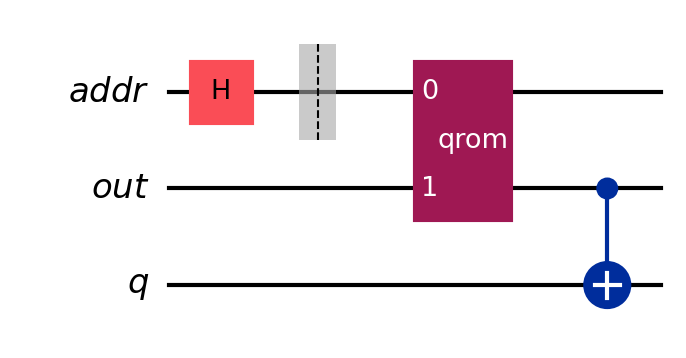
\includegraphics[width=0.9\textwidth]{assets/qrom_usage.png}
	\caption{A QROM applied on a circuit in which all its possible address are put in superposition, meaning that every mapping state has some chance of appearing in the $out$ qubit. After that, the resulting state can be used for further operations.} 
	\label{QROMUsage}
\end{figure}

Although it's a very simple device, due to the no-cloning-theorem, it's not possible to copy internal values and add it on different qubits. Because of that fact, we can only use the state as a entanglement source, or apply a quantum teleportation protocol to transfer the state from a qubit to another one. Also, this kind of memory can become really large depending on its goal, and is required to be reapplied each time a new value is needed.

These behaviors can hinder our ability to create a memory able to both read and write data, so, being able to structure of a QRAM in this case relies entirely on quantum teleportation. In the implemented protocol, it requires $n$ qubits for both data and address bus, however this one can handle only one address/data per qubit, so to handle $m$ addresses are required $m$ qubits.

\pagebreak

\begin{figure}[ht]
	\centering
	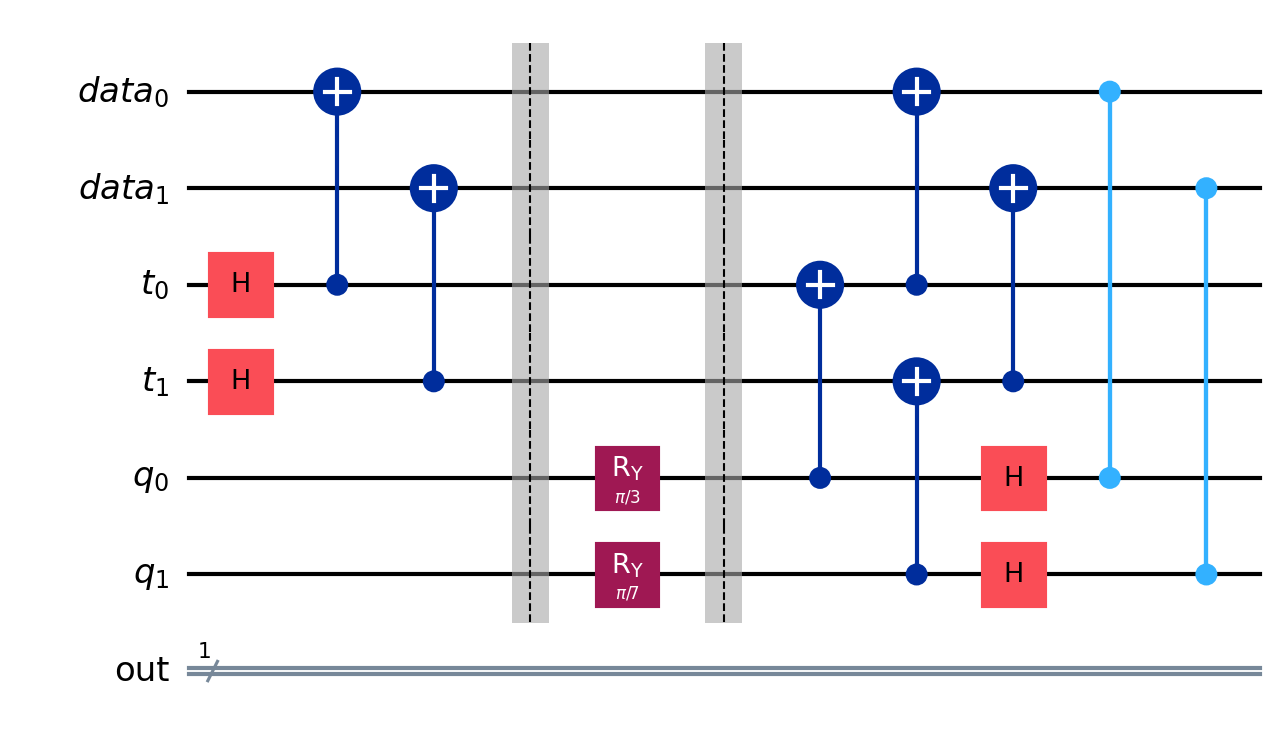
\includegraphics[width=0.9\textwidth]{assets/qram.png}
	\caption{A QRAM with $2$ qubits for data/addresses. In this example, the first $n$ data qubits act both as data and address. However, to teleport their states, additional $t$  qubits were added being in total $2*n$ qubits in the QRAM circuit. With that, our circuit qubits $q$ are prepared with some arbitrary states we want to save, then the teleportation protocol is applied and the previous stored data is removed from the circuit and moved to the QRAM domain.}
\end{figure}

Comparing this implementation with previous one, we have similar characteristics, once both QRAM and QROM can't have their values copied due to the no-cloning-theorem. However, this one doesn't require reapplication for writing and retrieving values, once they
were pre-applied at each data qubit. Also, it's possible to overwrite and interfere over data estates, so it's possible to reduce the memory size just managing stored values (Interference could also be done in the QROM just applying interference in the target qubits after calling for some address).

After finishing this project, we can conclude that it's possible to create some sort of memorization inside a circuit. Nevertheless, as retreaded at \cite{jaques2023qram} and \cite{Giovannetti_2008}, these devices are far away from real applications. Even using the circuits shown above, the real usage is not simple and practical, being needed many re-applications, clever data managing protocols and requiring a giant qubits overhead. It's also affected by several quantum implications that reduce its usefulness, like: no-cloning, decoherence, errors, etc.
Due to that, the best approach could be implementing a memory at hardware level \cite{jaques2023qram}, using peripheral devices to connect with it on software and them save or retrieve data when needed.
Based on this discussion, it's possible to conclude that, although it's possible to create memory circuits for small use cases, bigger ones are far from real.


\section{Conclusions}\label{conclusions}

With this work, it's evident that Quantum Computing has a big potential for the future. However, the lack of hardware capabilities and some quantum effects affect the real use cases for this new computing paradigm now.
As already shown by many researches in areas like: chemistry, physics, cryptograph, optimization, etc; Quantum computing can be the next breakthrough in technology and a decisive point for many companies around the world.
Nonetheless, during NISQ era, to increase the usefulness of such technology, it's still required using classical computing along with it to improve its capabilities. 

In conclusion, it's possible to take advantage of quantum computing now for some problems we know classically, but first, it's needed to investigate if there are some quantum factors that can improve the results. If positive, applying the hybrid approach it's, probably, the best solution for your problem, once you can trust on error mitigation for a small sample and then let the classical computing do its work in analyzing the output data.

\bibliography{references}

\end{document}
